\chapter{Конструкторская часть}

В этой части представляются требования к программе, алгоритм визуализации сцены, выбранные типы и структуры данных, диаграмма классов.

\section{Требования к программе}

Программа должна обладать графическим интерфейсом, который позволит пользователю:
\begin{itemize}[label=--]
	\item изменять геометрические и спектральные характеристики модели многогранника;
	\item изменять положение модели многогранника в пространстве;
	\item изменять положение камеры в пространстве;
	\item изменять режим отображения сцены между <<каркасным>>, <<реалистичным>>, <<световым>> и <<теневым>>, отображающими каркасы моделей, линии пересечения моделей, сцену с учётом освещения и сцену с тенями, возникающими от освещения, соответственно.
\end{itemize}

Разработанная программа должна выполнять следующие требования:
\begin{itemize}[label=--]
	\item источник света должен создаваться при запуске;
	\item в пространстве может быть только один источник света;
	\item в пространстве может быть только одна камера;
	\item программа обязана правильно обрабатывать некорректные вводимые данные.
\end{itemize}

\section{Общий алгоритм визуализации сцены}

На рисунке~\ref{fig:scene-visualization} представлен алгоритм, который генерирует изображение. Он принимает на вход геометрические и спектральные параметры моделей, характеристики камеры, данные об источнике света и его спектральные свойства, а на выходе предоставляет визуализированную сцену на экране.

\begin{figure}[h] 
	\centering
	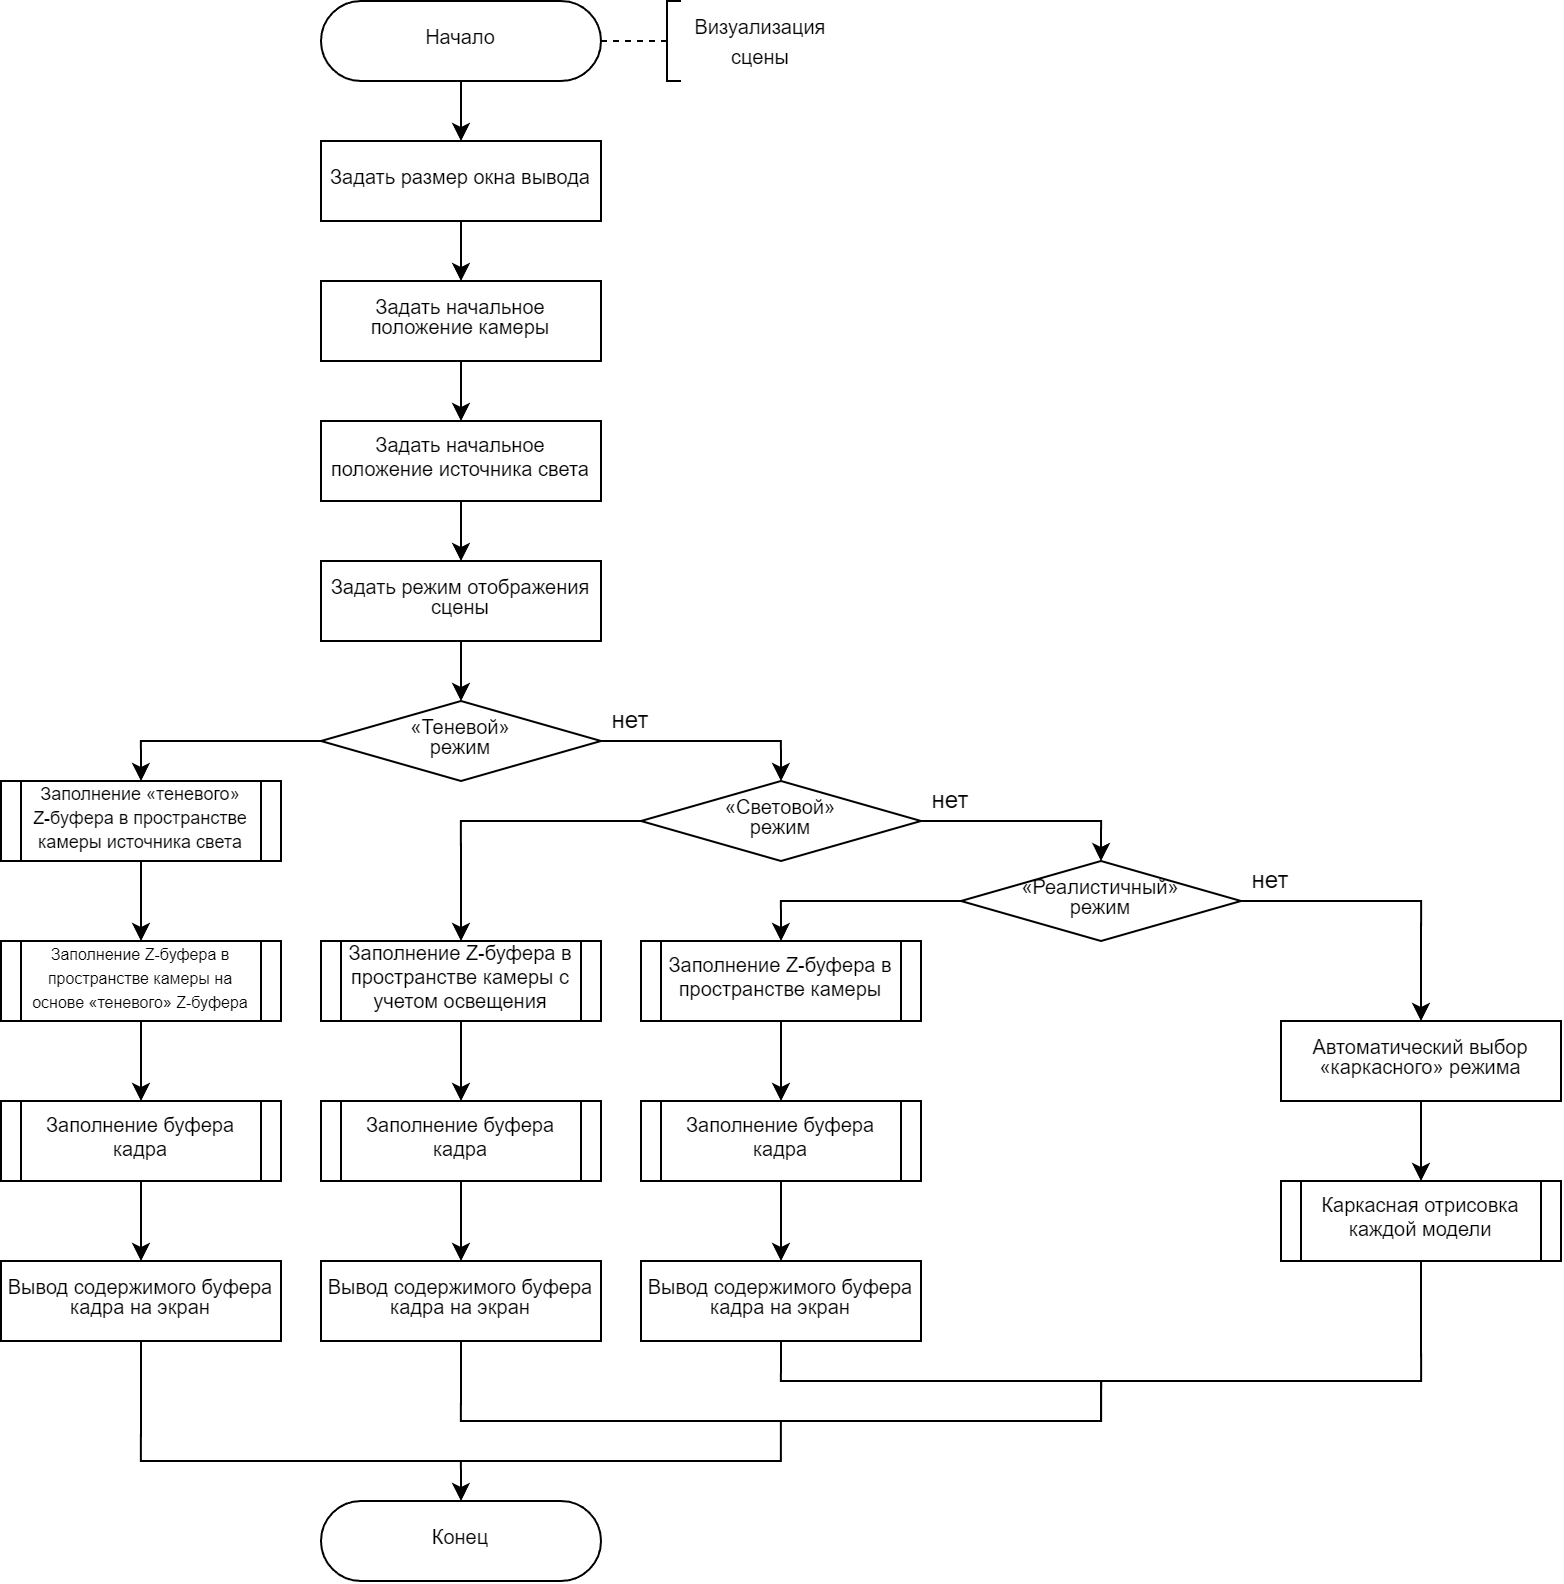
\includegraphics[width=1\textwidth]{images/scene-visualization.png}
	\caption{Общий алгоритм визуализации сцены} 
	\label{fig:scene-visualization} 
\end{figure}

\clearpage

Более подробный алгоритм визуализации сцены в <<теневом>> режиме отображения сцены при инициализированной сцене представлен на рисунке~
\ref{fig:shadow-mod}.
\begin{figure}[h] 
	\centering
	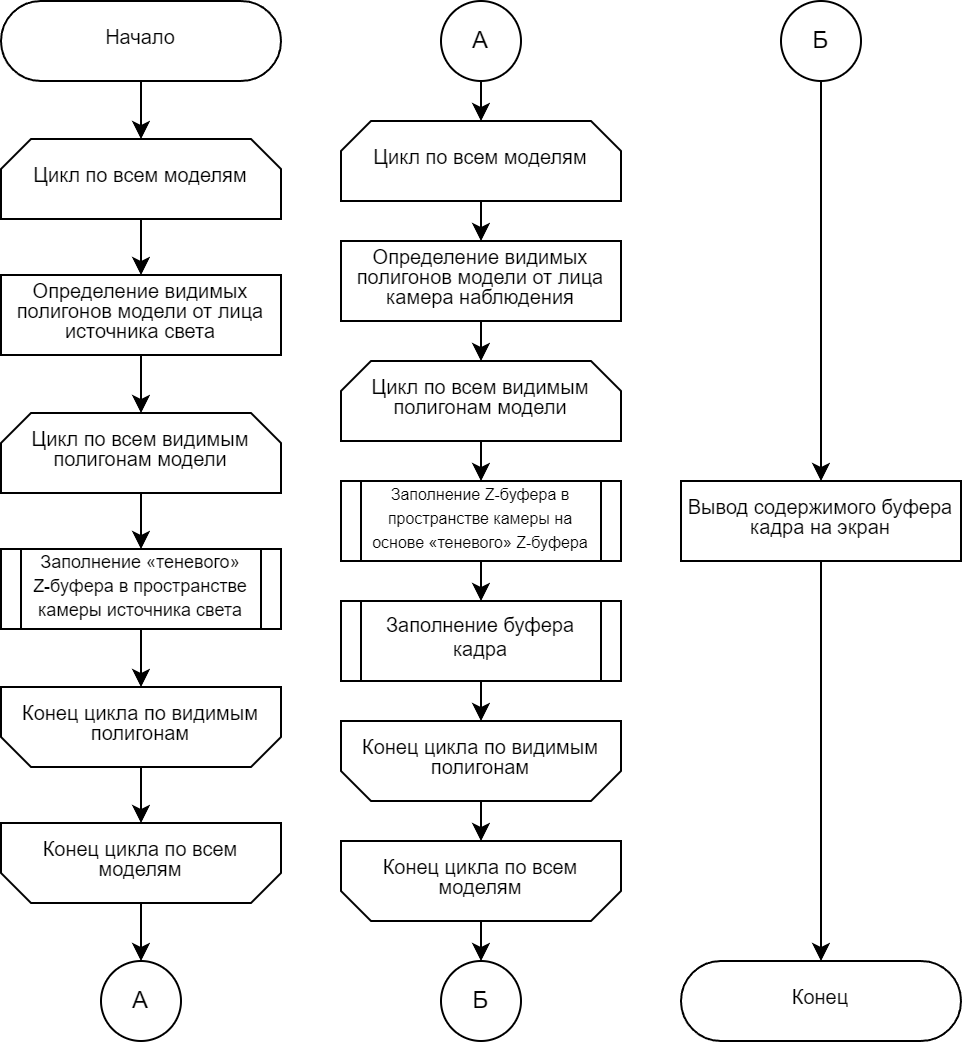
\includegraphics[width=1\textwidth]{images/shadow-mod.png}
	\caption{Общий алгоритм визуализации сцены в <<теневом>> режиме при инициализированной сцене} 
	\label{fig:shadow-mod} 
\end{figure}

\clearpage

Более подробный алгоритм визуализации сцены в <<световом>>, <<реалистичном>> и <<каркасном>> режимах отображения сцены при инициализированной сцене представлены на рисунке~\ref{fig:other-mods}.
\begin{figure}[h] 
	\centering
	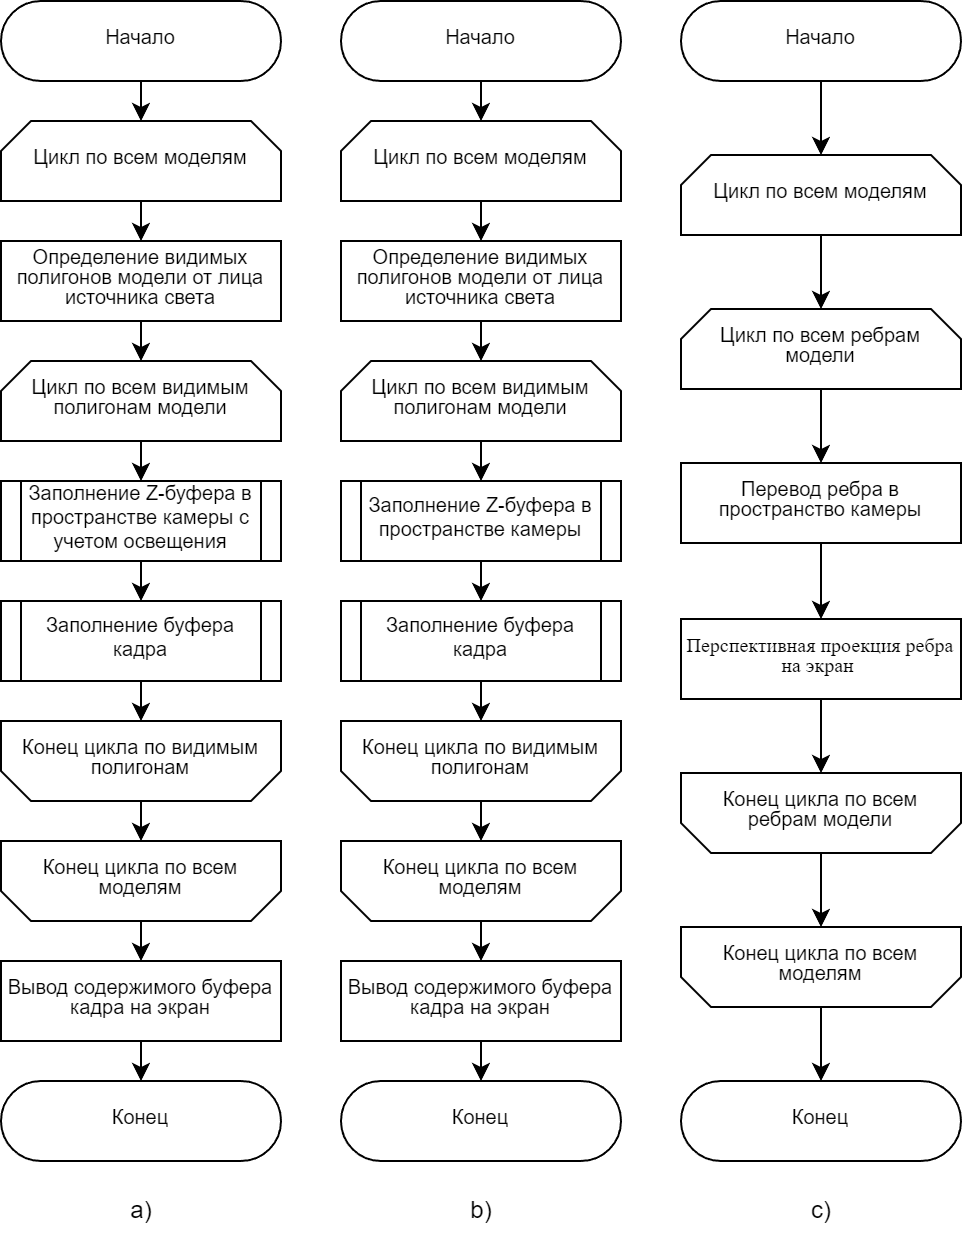
\includegraphics[width=0.8\textwidth]{images/other-mods.png}
	\caption{Общий алгоритм визуализации сцены в иных режимах при инициализированной сцене: <<световой>> (a), <<реалистичный>> (b), <<каркасный>> (c)} 
	\label{fig:other-mods} 
\end{figure}

\clearpage

\section{Афинные преобразования}

Для изменения положения модели в пространстве можно использовать следующие преобразования: перемещение и поворот~\cite{lit15}. Каждое из этих преобразований может быть представлено в виде матрицы:
\begin{enumerate}
	\item перемещение вдоль координатных осей $O_X$, $O_Y$ и $O_Z$ соответственно на величины $d_x$, $d_y$, $d_z$:
	\begin{equation}
		\begin{pmatrix}
			1 & 0 & 0 & 0 \\
			0 & 1 & 0 & 0 \\
			0 & 0 & 1 & 0 \\
			d_x & d_y & d_z & 1
		\end{pmatrix}
	\end{equation}
	\item поворот вокруг координатных осей $O_X$, $O_Y$ и $O_Z$ на угол $\theta$:
	\begin{equation}
		R = R_X \cdot R_Y \cdot R_Z
	\end{equation}
	где $R$ -- матрица поворота, $R_X$ матрица поворота вокруг оси $O_X$ на угол $\theta$, $R_Y$ -- матрица поворота вокруг оси $O_Y$ на угол $\theta$, $R_Z$ -- матрица поворота вокруг оси $O_Z$ на угол $\theta$.
	\begin{itemize}[label=--]
		\item поворот вокруг оси $O_X$ на угол $\theta$:
		\begin{equation}
			\begin{pmatrix}
				1 & 0 & 0 & 0 \\
				0 & cos(\theta) & sin(\theta) & 0 \\
				0 & -sin(\theta) & cos(\theta) & 0 \\
				0 & 0 & 0 & 1
			\end{pmatrix}
		\end{equation}
		\item поворот вокруг оси $O_Y$ на угол $\theta$:
		\begin{equation}
			\begin{pmatrix}
				cos(\theta) & 0 & -sin(\theta) & 0 \\
				0 & 1 & 0 & 0 \\
				sin(\theta) & 0 & cos(\theta) & 0 \\
				0 & 0 & 0 & 1
			\end{pmatrix}
		\end{equation}
		\item поворот вокруг оси $O_Z$ на угол $\theta$:
		\begin{equation}
			\begin{pmatrix}
				cos(\theta) & sin(\theta) & 0 & 0 \\
				-sin(\theta) & cos(\theta) & 0 & 0 \\
				0 & 0 & 1 & 0 \\
				0 & 0 & 0 & 1
			\end{pmatrix}
		\end{equation}
	\end{itemize}
\end{enumerate}

\section{Камера}

Камера отвечает за захват и отображение части трёхмерной сцены на двумерную поверхность~\cite{lit12}. Она определяет, как объекты будут видны зрителю, а также управляет параметрами визуализации, такими как угол обзора.

\subsection{Пирамида видимого пространства}

Пирамида видимого пространства (\textit{англ. viewing frustum}) представляет собой объем, в пределах которого объекты могут быть видимы камерой~\cite{lit12}. Этот объем имеет форму усеченной пирамиды (рис. \ref{fig:viewing-frustum}) и определяется несколькими ключевыми параметрами:
\begin{itemize}[label=--]
	\item ближняя плоскость: плоскость, находящаяся на определенном расстоянии от камеры, перед которой объекты начинают отображаться. Объекты, находящиеся ближе, не будут видны;
	\item дальняя плоскость: плоскость, за которой объекты не отображаются;
	\item поле зрения (\textit{англ. field of view}): угол, под которым камера охватывает сцену. Поле зрения влияет на то, насколько широко камера может видеть, и определяет степень искажения объектов в зависимости от их расстояния до камеры.
\end{itemize}

Пирамида видимого пространства позволяет игнорировать объекты вне этого объема, что увеличивает скорость рендеринга.

\clearpage

\begin{figure}[h] 
	\centering
	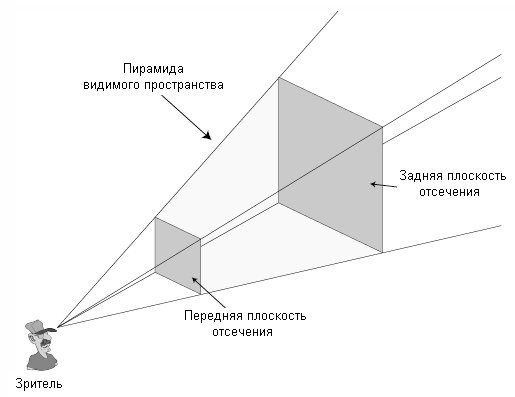
\includegraphics[width=0.7\textwidth]{images/viewing-frustum.png}
	\caption{Пирамида видимого пространства} 
	\label{fig:viewing-frustum} 
\end{figure}

\subsection{Пространство модели}

Пространство модели -- это локальная система координат, в которой располагается конкретный объект сцены~\cite{lit14}. В этом пространстве объект имеет координаты, которые определяют его положение, ориентацию и масштаб относительно своей собственной системы координат. 

Пусть вершина $V_L$ имеет однородные координаты $(x_L, y,_L z_L, 1)$ в пространстве модели, тогда её можно описать с помощью матрицы:
\begin{equation}
	V_L = 
	\begin{pmatrix}
		x_L \\
		y_L \\
		z_L \\
		1
	\end{pmatrix}
	\label{eq:local-vertex}
\end{equation}

\subsection{Мировое пространство}

Мировое пространство -- это система координат, в которой расположены все объекты сцены~\cite{lit14}. В этом пространстве каждое тело имеет свои координаты, определяющие его положение, ориентацию и масштаб. Мировое пространство позволяет организовать объекты в сцене.

Для перевода модели из её пространства в мировое необходима матрица перевода. Для её формирования необходимо составить матрицу перемещения модели относительно начала мировой системы координат и матрицу поворота модели относительно её центра.
\begin{equation}
	W = M_W \cdot R_W
\end{equation}
где $W$ -- матрица перевода модели из её пространства в мировое, $M_W$ -- матрица перемещения, $R_W$ -- матрица поворота.

Чтобы перевести вершину $V_L$ (\ref{eq:local-vertex}) из её локального пространства в мировое, её нужно умножить на матрицу перевода $W$:
\begin{equation}
	V_W = W \cdot V_L
	\label{eq:world-vertex}
\end{equation}
где $V_W$ -- матричная запись вершины $V_L$, переведённой из её локального пространства в мировое и имеющей однородные координаты $(x_W, y_W, z_W, w_W)$, $W$ -- матрица перевода модели из её пространства в мировое.

\subsection{Пространство камеры}

Пространство камеры -- это система координат, в которой камера воспринимает объекты~\cite{lit13, lit14}. Основные компоненты пространства камеры включают:

\begin{itemize}[label=--]
	\item положение камеры $P$: определяет, где находится камера в мировом пространстве;
	\item ориентация камеры $\vec{D}$: направление взгляда камеры, задаваемое вектором;
	\item cистема координат $\vec{D}, \vec{U}, \vec{R}$: устанавливает оси $O_X$, $O_Y$ и $O_Z$ для камеры, где ось $\vec{D}$ направлена вперед (ампликата), ось $\vec{U}$ -- вверх (ордината), а ось $\vec{R}$ -- вправо (абсцисса).
	\begin{equation}
		\vec{R} = \vec{D} \times O_Y \\
	\end{equation}
	\begin{equation}
		\vec{U} = \vec{D} \times \vec{R}
	\end{equation}
\end{itemize}

Для перевода модели из мирового пространства в пространство камеры необходима матрица перевода. Для её формирования необходимо составить матрицу перемещения камеры относительно начала мировой системы координат и матрицу поворота камеры в мировом пространстве.
\begin{equation}
	M_C = 
	\begin{pmatrix}
		1 & 0 & 0 & 0 \\
		0 & 1 & 0 & 0 \\
		0 & 0 & 1 & 0 \\
		-P_x & -P_y & -P_z & 1
	\end{pmatrix}
\end{equation}
где $M_C$ -- матрица перемещения камеры относительно начала мировой системы координат, $P$ -- положение камеры в мировом пространстве.

\begin{equation}
	R_C = 
	\begin{pmatrix}
		\vec{R}_x & \vec{U}_x & \vec{D}_x & 0 \\
		\vec{R}_y & \vec{U}_y & \vec{D}_y & 0 \\
		\vec{R}_z & \vec{U}_z & \vec{D}_z & 0 \\
		0 & 0 & 0 & 1 
	\end{pmatrix}
\end{equation}
где $R_C$ -- матрица поворота камеры в мировом пространстве, $\vec{R}$ -- абсцисса системы координат камеры, $\vec{U}$ -- ордината системы координат камеры, $\vec{D}$ -- направление взгляда камеры (ампликата системы координат камеры).

\begin{equation}
	C = M_C \cdot R_C
\end{equation}
где $C$ -- матрица перевода модели из мирового пространства в пространство камеры, $M_C$ -- матрица перемещения камеры относительно начала мировой системы координат, $R_C$ -- матрица поворота камеры в мировом пространстве.

Чтобы перевести вершину $V_W$ (\ref{eq:world-vertex}) из мирового пространства в пространство камеры, её нужно умножить на матрицу перевода:
\begin{equation}
	V_C = C \cdot V_W
	\label{eq:camera-vertex}
\end{equation}
где $V_C$ -- матричная запись вершины $V_W$, переведённой из мирового пространства в пространство камеры и имеющей однородные координаты $(x_C, y_C, z_C, w_C)$, $C$ -- матрица перевода модели из мирового пространства в пространство камеры. 

\subsection{Пространство отсечения}

Пространство отсечения -- это трехмерное пространство в виде куба, в котором все вершины объектов представлены в координатах, нормализованных в диапазоне от -1 до 1 для каждой из осей $O_X$, $O_Y$ и $O_Z$~\cite{lit14}. Если вершина после её перевода в пространство отсечения имеет какую-либо координату, значение которой не входит в промежуток от -1 до 1, то рендеринг этой вершины прекращается.

Для перевода модели из пространства камеры в пространство отсечения необходима матрица \textit{перспективной проекции}. Для её формирования нужны значения ширины и высоты экрана, вертикального угла обзора, расстояний до ближней и дальней плоскостей пирамиды видимого пространства.
\begin{equation}
	P = 
	\begin{pmatrix}
		\frac{1}{tg(\frac{\gamma}{2}) \cdot \frac{W}{H}} & 0 & 0 & 0 \\
		0 & \frac{1}{tg(\frac{\gamma}{2})} & 0 & 0 \\
		0 & 0 & -\frac{F + N}{F - N} & -2\frac{F \cdot N}{F - N} \\
		0 & 0 & -1 & 0 
	\end{pmatrix}
	\label{eq:clip-matrix}
\end{equation}
где $P$ -- матрица перевода из пространства камеры в пространство отсечения, $\gamma$ -- вертикальный угол обзора, $W$ -- ширина экрана, $H$ -- высота экрана, $F$ -- расстояние до дальней плоскости пирамиды видимого пространства, $N$ -- расстояние до ближней плоскости пирамиды видимого пространства.

Запись матрицы $P$ (\ref{eq:clip-matrix}) можно упростить. Пусть $Z_y = \frac{1}{tg(\frac{\gamma}{2})}$, $R = \frac{W}{H}$, $Z_x = \frac{Z_y}{R}$, тогда:
\begin{equation}
	P = 
	\begin{pmatrix}
		Z_x & 0 & 0 & 0 \\
		0 & Z_y & 0 & 0 \\
		0 & 0 & -\frac{F + N}{F - N} & -2\frac{F \cdot N}{F - N} \\
		0 & 0 & -1 & 0 
	\end{pmatrix}
\end{equation}

Чтобы перевести вершину $V_C$ (\ref{eq:camera-vertex}) из пространства камеры в пространство отсечения, её нужно умножить на матрицу перевода:
\begin{equation}
	V_P = P \cdot V_C
	\label{eq:clip-vertex}
\end{equation}
где $V_P$ -- матричная запись вершины $V_C$, переведенной из пространства камеры в пространство отсечения и имеющей однородные координаты $(x_P, y_P, z_P, w_P)$, $P$ -- матрица перевода из пространства камеры в пространство отсечения.

Чтобы проверить принадлежность вершины $V_P$ (\ref{eq:clip-vertex}) пространству отсечения, её однородные координаты нужно нормализовать и проверить принадлежность их значений промежутку от -1 до 1:
\begin{equation}
	\begin{cases}
		-1 \le x_{NP} \le 1 \\
		-1 \le y_{NP}\le 1 \\
		-1 \le z_{NP} \le 1
	\end{cases}
\end{equation}
где $x_{NP} = \frac{x_P}{w_P}$ -- нормализованная координата $x_P$, $y_{NP} = \frac{y_P}{w_P}$ -- нормализованная координата $y_P$, $z_{NP} = \frac{z_P}{w_P}$ -- нормализованная координата $x_P$.

\subsection{Пространство экрана}

Пространство экрана -- это координатная система, в которой трехмерные объекты сцены отображаются как двумерные изображения на экране~\cite{lit13, lit14}. Данная координатная система определяется двумя осями $O_X$ и $O_Y$, направленными вправо и вниз соответственно, и имеет фиксированные размеры, которые зависят от разрешения экрана.

Для перевода вершины $V_P$ (\ref{eq:clip-vertex}) из пространства отсечения в пространство экрана, её вершины необходимо предварительно нормализовать. Пусть $V_{NP}$ -- нормализованная вершина $V_P$, имеющая однородные координаты $(x_{NP}, y_{NP}, \\ z_{NP}, 1)$, тогда:
\begin{equation}
	\begin{aligned}
		D_x &= (x_{NP} \cdot 0.5 + 0.5) \cdot W \\
		D_y &= (y_{NP} \cdot 0.5 + 0.5) \cdot H
	\end{aligned}
\end{equation}
где $D$ -- вершина $V_P$, переведенная из пространства отсечения в пространство экрана и имеющая координаты $(D_x, D_y)$, $W$ -- ширина экрана, $H$ -- высота экрана.

\subsection{Алгоритм получения изображения от лица камеры}

На рисунке~\ref{fig:camera-image} представлен алгоритм получения изображения модели на экране от лица камеры. Он принимает на вход вершины модели в её локальном пространстве, а на выходе предоставляет изображение вершин модели от лица камеры на экране.
\begin{figure}[h] 
	\centering
	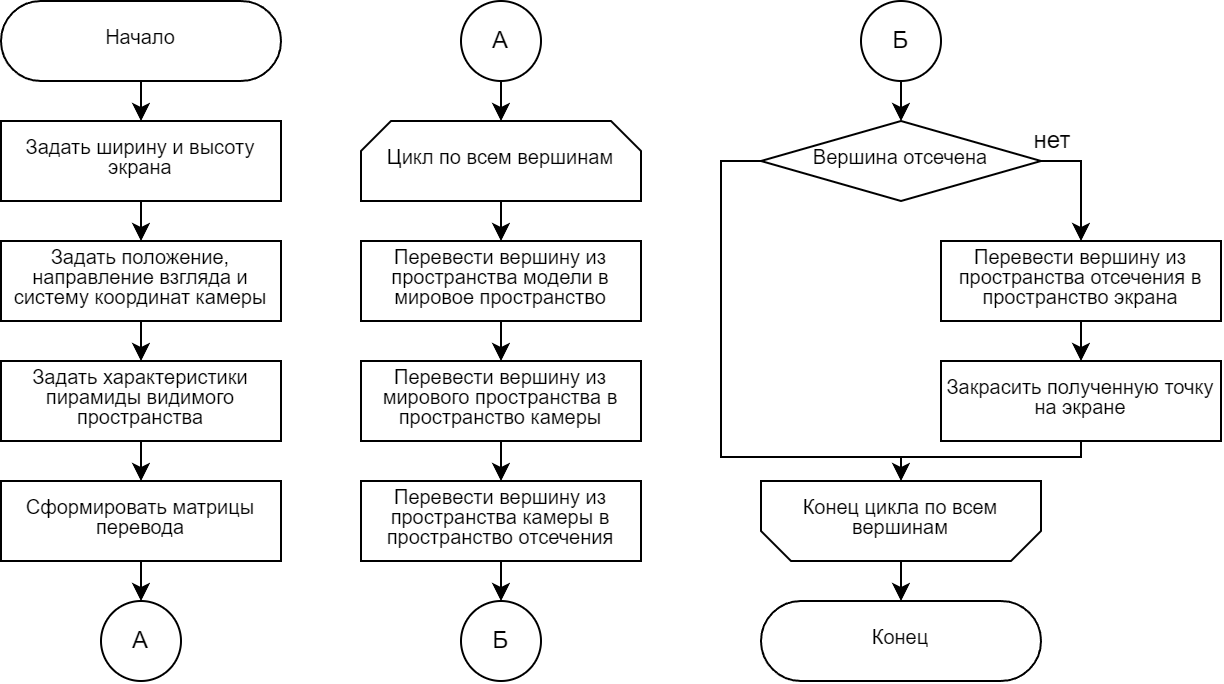
\includegraphics[width=1\textwidth]{images/camera-image.png}
	\caption{Алгоритм получения изображения модели на экране от лица камеры} 
	\label{fig:camera-image} 
\end{figure}
\begin{figure}[h] 
	\centering
	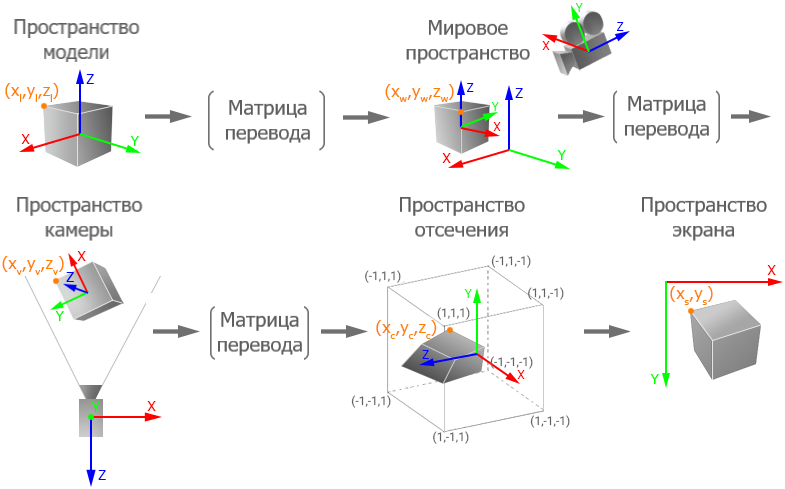
\includegraphics[width=1\textwidth]{images/space_transformations.png}
	\caption{Последовательный перевод модели из одного пространства в другое} 
	\label{fig:space-transformations} 
\end{figure}

\clearpage

\section{Невидимые грани}

Отбрасывание граней, которые не видны с точки зрения камеры, значительно ускоряет процесс рендеринга изображений~\cite{lit3}. Это связано с тем, что невидимые полигоны не требуют обработки, что позволяет сэкономить ресурсы. Чтобы определить, видима ли грань, используется следующая формула:
\begin{equation}
	(\vec{N}, \vec{V}) =
	\begin{cases}
		\geq 0, & \text{если грань видима} \\
		< 0, & \text{если грань невидима}
	\end{cases}
\end{equation}
где $\vec{N}$ -- вектор, перпендикулярный поверхности грани и направленный наружу от модели, $\vec{V}$ -- вектор, указывающий от камеры к любой точке на грани.

\section{Алгоритм Z-буфера}

Для применения алгоритма $Z$-буфера к модели необходимо определить все точки, принадлежащие полигону. Поскольку количество точек на полигоне бесконечно, под поиском всех точек подразумевается создание конечного набора точек, который адекватно аппроксимирует полигон при выводе на экран, обеспечивая непрерывность и избегая эффекта <<сетчатости>>.

Для эффективного рендеринга полигона необходимо предварительно определить его ограничивающую прямую призму. Это позволит установить конкретную область в трехмерном пространстве, в которой расположен полигон.

Пусть $P$ -- полигон, заданный вершинами $(P_1(x_1, y_1, z_1), P_2(x_2, y_2, z_2), \\ P_3(x_3, y_3, z_3), P_4(x_4, y_4, z_4))$, $B$ -- ограничивающая прямая призма, заданная диагональю $D$ с вершинами $(D_1(D_{1_x}, D_{1_y}, D_{1_z}), D_2(D_{2_x}, D_{2_y}, D_{2_z}))$, $B_1$ -- нижнее основание  призмы $B$, заданное вершинами $(A, B, C, D)$, $B_2$ -- верхнее основание призмы $B$, заданное вершинами $(A_1, B_1, C_1, D_1)$. 
\begin{equation}
	\begin{aligned}
		D_{1_x} = min(x_1, x_2, x_3, x_4) \\
		D_{1_y} = min(y_1, y_2, y_3, y_4) \\
		D_{1_z} = min(z_1, z_2, z_3, z_4) 
	\end{aligned}
\end{equation} 
\begin{equation}
	\begin{aligned}
		D_{2_x} = max(x_1, x_2, x_3, x_4) \\
		D_{2_y} = max(y_1, y_2, y_3, y_4) \\
		D_{2_z} = max(z_1, z_2, z_3, z_4) 
	\end{aligned}
\end{equation}

Имея координаты вершин диагонали $D$, можно определить координаты всех вершин ограничивающей призмы $B$:
\begin{equation}
	\begin{aligned}
		A(D_{1_x}, D_{1_y}, D_{1_z}),
		B(D_{2_x}, D_{1_y}, D_{1_z}), \\
		C(D_{2_x}, D_{2_y}, D_{1_z}),
		D(D_{1_x}, D_{2_y}, D_{1_z})
	\end{aligned}
\end{equation}
\begin{equation}
	\begin{aligned}
		A_1(D_{1_x}, D_{1_y}, D_{2_z}),
		B_1(D_{1_x}, D_{2_y}, D_{2_z}), \\
		C_1(D_{2_x}, D_{2_y}, D_{2_z}), 
		D_1(D_{2_x}, D_{1_y}, D_{2_z}) 
	\end{aligned}
\end{equation}

Для формирования набора точек, принадлежащих полигону, можно проанализировать множество внутренних точек ограничивающей призмы с заданной точностью и проверить каждую из них на принадлежность полигону. Однако, более эффективным подходом будет анализ множества точек с заданной точностью, полученных из проекции ограничивающей призмы на плоскость $XY$. Для каждой из этих точек можно вычислить координату $z$ с использованием уравнения плоскости (\ref{eq:plane-eq}), которой принадлежит полигон. Это значительно сократит количество рассматриваемых трехмерных точек и позволит избежать необходимости проверки каждой точки на принадлежность плоскости полигона.

Пусть $P$ -- полигон, заданный $n$ вершинами $(P_1, P_2, \cdots, P_n)$, $A$ -- точка в плоскости полигона. Для определения принадлежности точки $A$ полигону $P$ можно использовать метод, основанный на проверке видимости точки относительно всех сторон полигона. Данный метод осуществляется в два этапа:
\begin{enumerate}
	\item определение внутренней нормали к каждой из сторон: для определения внутренней нормали $\vec{N_i}$ к стороне $P_iP_{i+1}$ предварительно вычисляется нормаль $\vec{V}$ к полигону.
	\begin{equation}
		\vec{V} = \overline{P_{i-1}P_{i}} \times \overline{P_{i}P_{i+1}}
	\end{equation}
	\begin{equation}
		\vec{N_i} = \overline{P_iP_{i+1}} \times \vec{V}
	\end{equation}
	
	\item проверка видимости относительно каждой стороны полигона: для каждой стороны $P_iP_{i+1}$ вычисляется вектор $W_i = \overline{Af_i}$, где $f_i$ -- произвольная точка на стороне $P_iP_{i+1}$. Затем вычисляется скалярное произведение $\vec{N_i} \cdot \vec{W_i}$. Если условие $\vec{N_i} \cdot \vec{W_i} > 0$, то точка $A$ находится на видимой стороне относительно текущей стороны. Если для всех сторон полигона это условие выполняется, то точка принадлежит полигону.
\end{enumerate}

На рисунке~\ref{fig:set-points} представлен алгоритм получения множества точек полигона. Он принимает на вход вершины полигона, а на выходе предоставляет массив трехмерных точек, принадлежащих полигону.

\begin{figure}[h] 
	\centering
	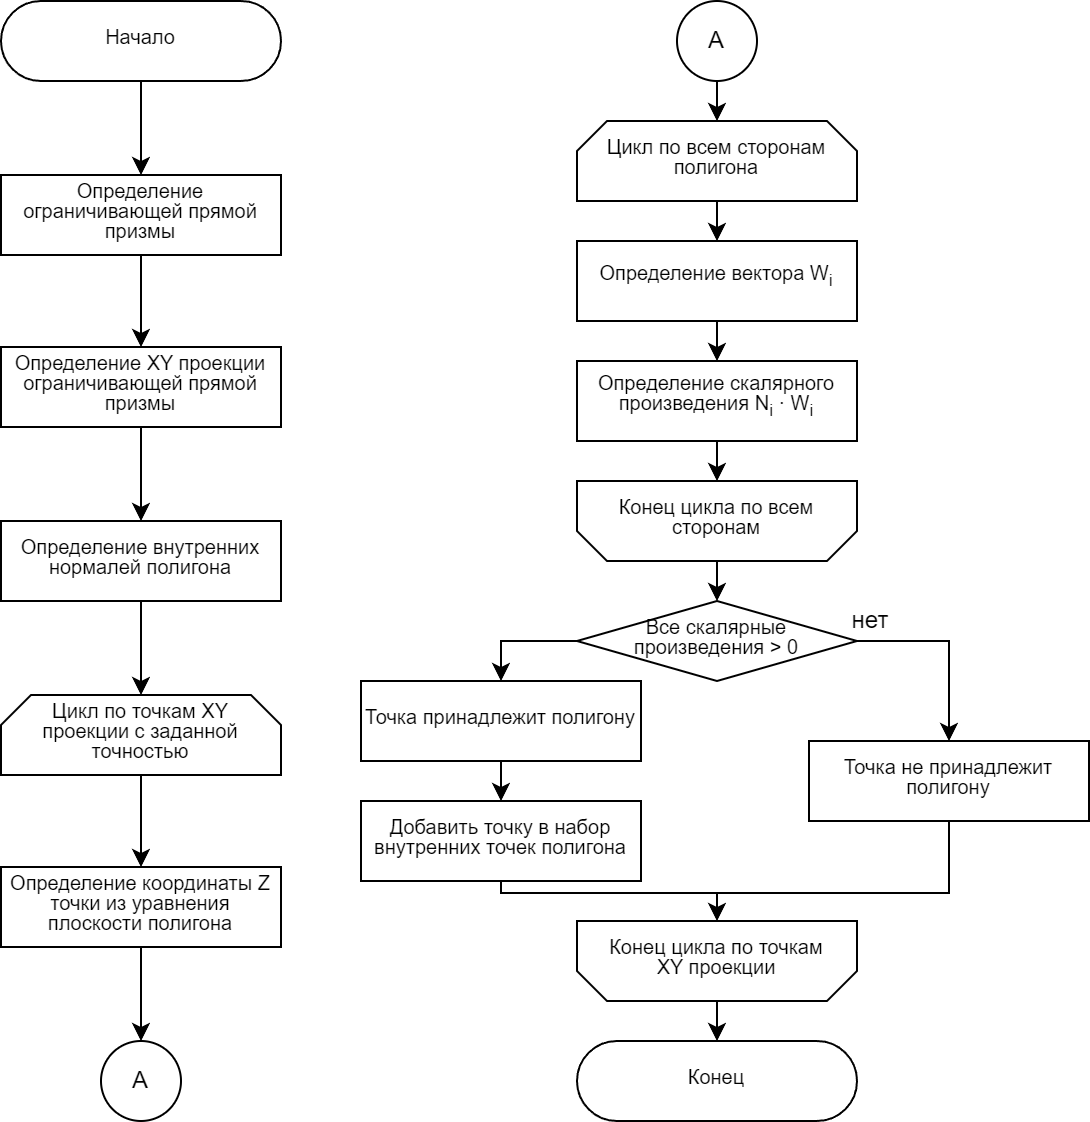
\includegraphics[width=1\textwidth]{images/points-set.png}
	\caption{Алгоритм получения множества точек полигона} 
	\label{fig:set-points} 
\end{figure}

На рисунке~\ref{fig:z-buffer} представлен алгоритм $Z$-буфера. Он принимает на вход геометрические параметры моделей, характеристики камеры, а на выход предоставляет изображение множества моделей сцены от лица камеры на экране.

\begin{figure}[h] 
	\centering
	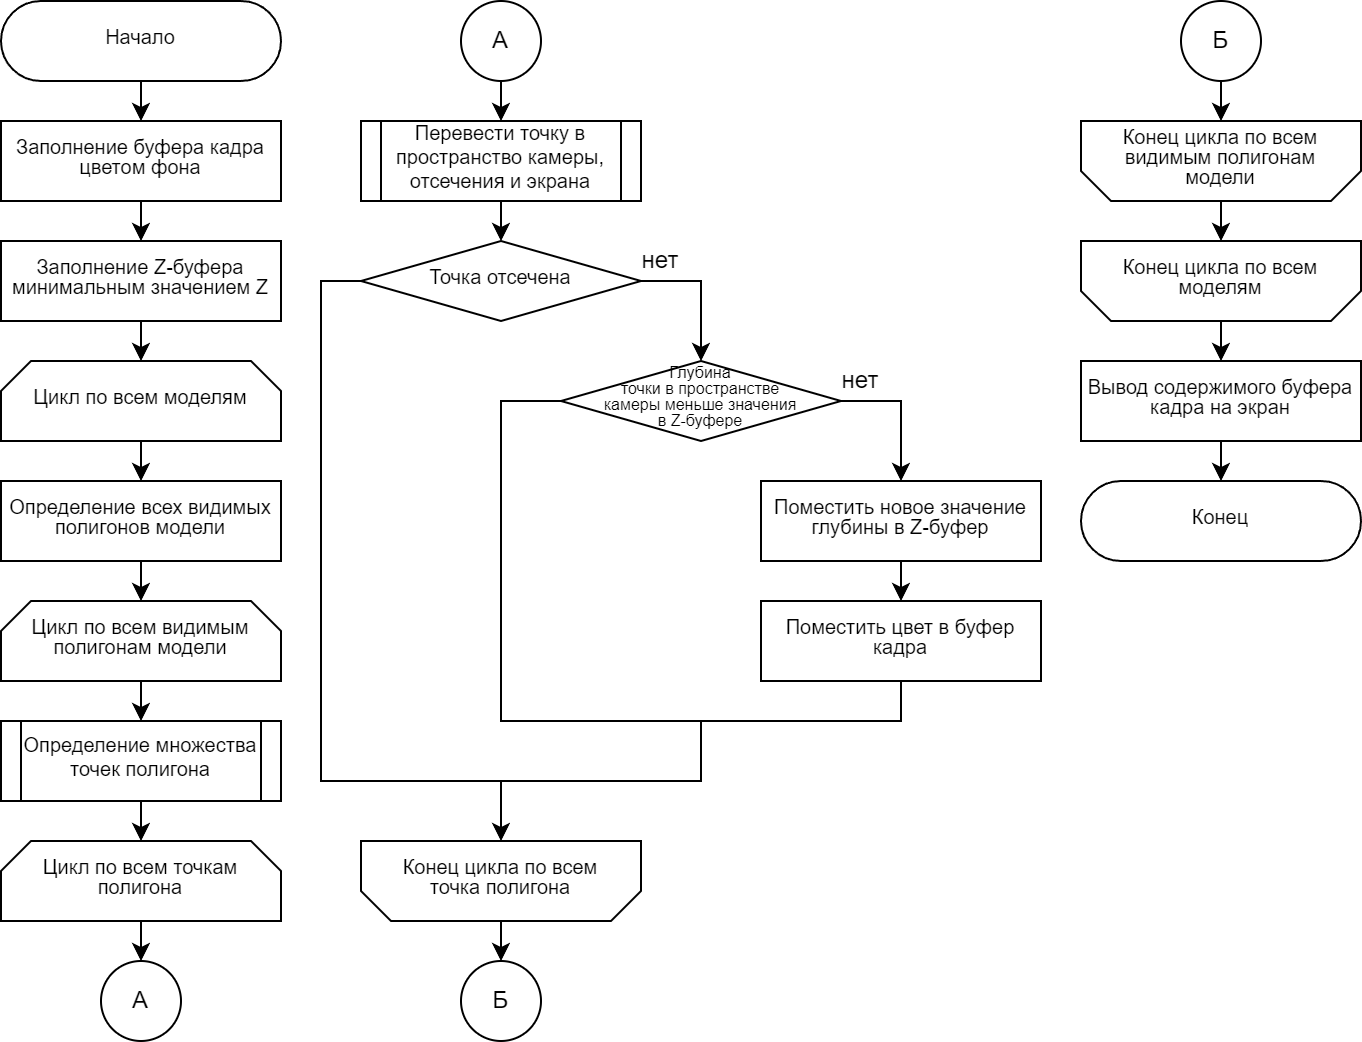
\includegraphics[width=1\textwidth]{images/z-buffer.png}
	\caption{Алгоритм Z-буфера} 
	\label{fig:z-buffer} 
\end{figure}

\section{Выбор типов и структур данных}

Использующиеся в программе структуры данных:
\begin{enumerate}
	\item модель многогранника, включающая в себя:
	\begin{itemize}[label=--]
		\item массив вершин;
		\item массив ребер;
		\item массив полигонов;
		\item геометрические характеристики;
		\item спектральные характеристики;
		\item цвет граней.
	\end{itemize}
	\item источник света, включающий в себя:
	\begin{itemize}[label=--]
		\item положение в пространстве;
		\item направление потока света.
	\end{itemize}
	\item сцена, включающая в себя:
	\begin{itemize}[label=--]
		\item массив моделей;
		\item источник света.
	\end{itemize}
	\item камера, включающая в себя:
	\begin{itemize}[label=--]
		\item положение в пространстве;
		\item направление просмотра;
		\item система координат, задаваемая тремя ортогональными векторами;
		\item характеристики пирамиды видимого пространства.
	\end{itemize}
	\item экран, включающий в себя:
	\begin{itemize}[label=--]
		\item сцену;
		\item камеру;
		\item значения сторон экрана.
	\end{itemize}
\end{enumerate}

\section{Диаграмма классов}

На рисунке~\ref{fig:class-diagram} представлена диаграмма классов.

\clearpage

\begin{figure}[h] 
	\centering
	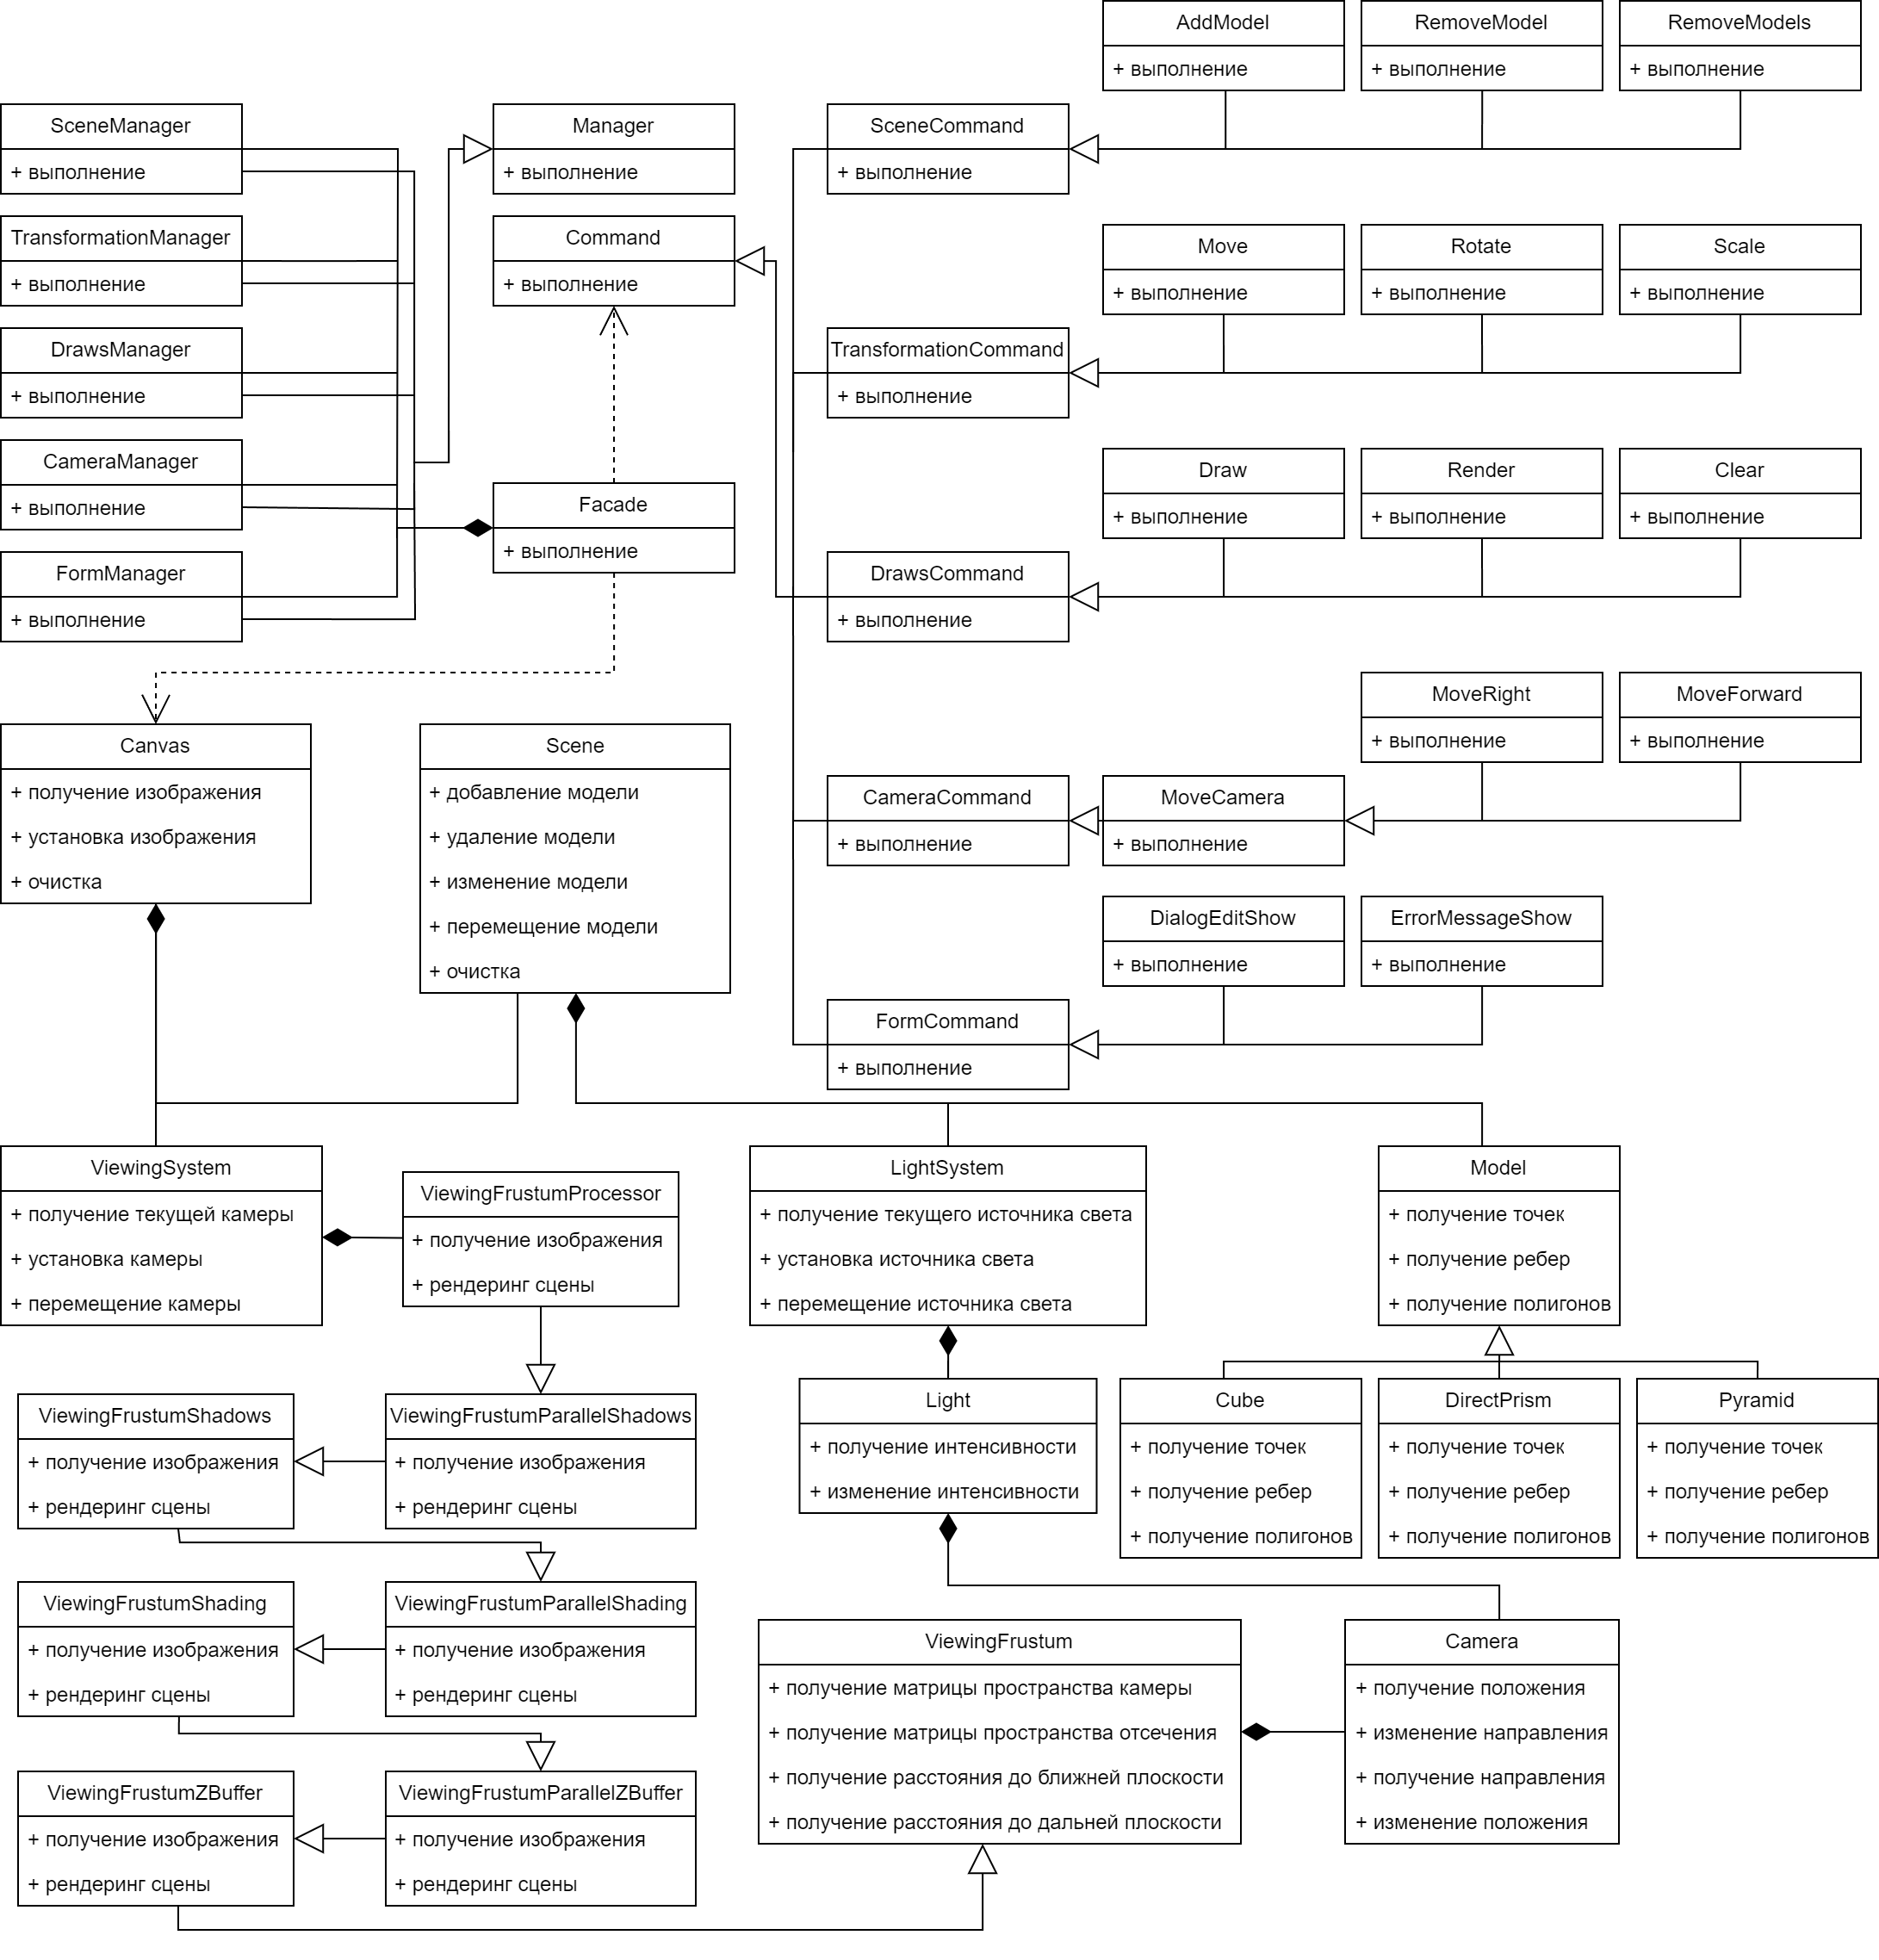
\includegraphics[width=1\textwidth]{images/class-diagram.png}
	\caption{Диаграмма классов} 
	\label{fig:class-diagram} 
\end{figure}

\section{Вывод}

В конструкторской части работы были представлены требования к программе, алгоритм визуализации сцены, выбранные типы и структуры данных, диаграмма классов.

\clearpage
